\documentclass[t]{beamer}
\usepackage{fontawesome5}
\usepackage{physics}
\usepackage{amsmath}
\usepackage{mathtools}
\usepackage{tikz}
\usepackage{mathdots}
\usepackage{yhmath}
\usepackage{nicematrix}
\usepackage{cancel}
\usepackage{color}
\usepackage{siunitx}
\usepackage{array}
\usepackage{multirow}
\usepackage[version=4]{mhchem}
\usepackage{amssymb}
\usepackage{textcomp, gensymb}
\usepackage{pifont}
\newcommand{\cmark}{\ding{51}}%
\newcommand{\xmark}{\ding{55}}%
\usepackage{tabularx}
\usepackage{extarrows}
\usepackage{booktabs}
\usetikzlibrary{fadings}
\usetikzlibrary{patterns}
\usetikzlibrary{shadows.blur}
\usetikzlibrary{shapes}
\usepackage[style=authoryear,backend=bibtex]{biblatex}
\addbibresource{arpes.bib}
\renewcommand{\footnotesize}{\scriptsize}
\usepackage{listings}
\usepackage{hyperref}

\newcommand{\pair}[1]{\langle #1 \rangle}
\DeclareMathOperator{\ee}{e}
\DeclareMathOperator{\ii}{i}

\newcommand{\concept}[1]{\textbf{#1}}
\newcommand*{\abinitio}{\textit{ab initio}}
\newcommand{\shortcode}[1]{\texttt{#1}}

\newcommand*{\Gammae}{\Gamma_{\text{e}}}
\newcommand*{\Gammag}{\Gamma_{\text{g}}}
\newcommand*{\omegae}{\omega_{\text{e}}}
\newcommand*{\omegag}{\omega_{\text{g}}}
\newcommand*{\omegaeg}{\omega_{\text{eg}}}
\newcommand*{\ptwfc}[2]{\psi^{(#2)}_{#1}}
\newcommand*{\mueg}{\mu_{\text{eg}}}
\newcommand*{\muge}{\mu_{\text{ge}}}
\newcommand*{\Ezzero}{E_{z0}}
\newcommand*{\kete}{\ket*{\text{e}}}
\newcommand*{\ketg}{\ket*{\text{g}}}
\newcommand*{\coeffe}{c_{\text{e}}}
\newcommand*{\coeffg}{c_{\text{g}}}
\newcommand*{\pope}{p_{\text{e}}}
\newcommand*{\popg}{p_{\text{g}}}

\newcommand\blfootnote[1]{%
\begingroup
\renewcommand\thefootnote{}\footnote{#1}%
\addtocounter{footnote}{-1}%
\endgroup
}

%Information to be included in the title page:
\title{Cavity QED}
\subtitle{Quantum light-matter interaction to the extreme}
\author{Jinyuan Wu}

\usetheme{metropolis}   

\begin{document}

\maketitle

\begin{frame}
\frametitle{When do all effective theories of light or matter fail? }

\begin{center}
    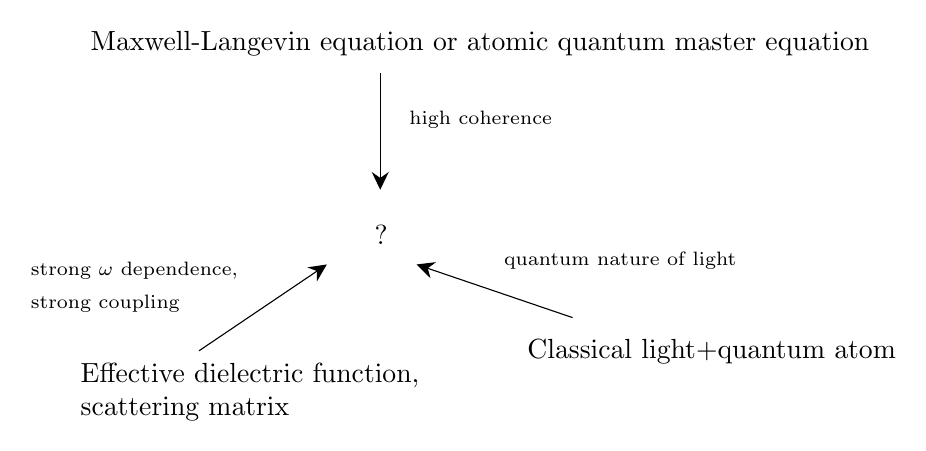
\begin{tikzpicture}[x=0.75pt,y=0.75pt,yscale=-0.8,xscale=0.8]
        %uncomment if require: \path (0,300); %set diagram left start at 0, and has height of 300
        
        %Straight Lines [id:da8835458472145681] 
        \draw    (256,78) -- (256,145.28) ;
        \draw [shift={(256,148.28)}, rotate = 270] [fill={rgb, 255:red, 0; green, 0; blue, 0 }  ][line width=0.08]  [draw opacity=0] (10.72,-5.15) -- (0,0) -- (10.72,5.15) -- (7.12,0) -- cycle    ;
        %Straight Lines [id:da7971466628067554] 
        \draw    (146.83,245.28) -- (221.35,194.96) ;
        \draw [shift={(223.83,193.28)}, rotate = 145.97] [fill={rgb, 255:red, 0; green, 0; blue, 0 }  ][line width=0.08]  [draw opacity=0] (10.72,-5.15) -- (0,0) -- (10.72,5.15) -- (7.12,0) -- cycle    ;
        %Straight Lines [id:da8117487283986535] 
        \draw    (371.83,225.28) -- (280.67,194.25) ;
        \draw [shift={(277.83,193.28)}, rotate = 18.8] [fill={rgb, 255:red, 0; green, 0; blue, 0 }  ][line width=0.08]  [draw opacity=0] (10.72,-5.15) -- (0,0) -- (10.72,5.15) -- (7.12,0) -- cycle    ;
        
        % Text Node
        \draw (74,251) node [anchor=north west][inner sep=0.75pt]   [align=left] {Effective dielectric function,\\scattering matrix};
        % Text Node
        \draw (80,51) node [anchor=north west][inner sep=0.75pt]   [align=left] {Maxwell-Langevin equation or atomic quantum master equation};
        % Text Node
        \draw (272,99) node [anchor=north west][inner sep=0.75pt]   [align=left] {\footnotesize high coherence};
        % Text Node
        \draw (44,190) node [anchor=north west][inner sep=0.75pt]   [align=left] {\footnotesize strong $\displaystyle \omega $ dependence,\\ \footnotesize strong coupling};
        % Text Node
        \draw (343,237) node [anchor=north west][inner sep=0.75pt]   [align=left] {Classical light+quantum atom};
        % Text Node
        \draw (329,184) node [anchor=north west][inner sep=0.75pt]   [align=left] {\footnotesize quantum nature of light};
        % Text Node
        \draw (251,168) node [anchor=north west][inner sep=0.75pt]   [align=left] {?}; 
        \end{tikzpicture}        
\end{center}

\textbf{One scenario: in a cavity. }

\end{frame}

\section{Cavity and one atom}

\begin{frame}
\frametitle{Cavity quantum electrodynamics (cavity QED)}

\begin{center}
    \tikzset{every picture/.style={line width=0.75pt}} %set default line width to 0.75pt        

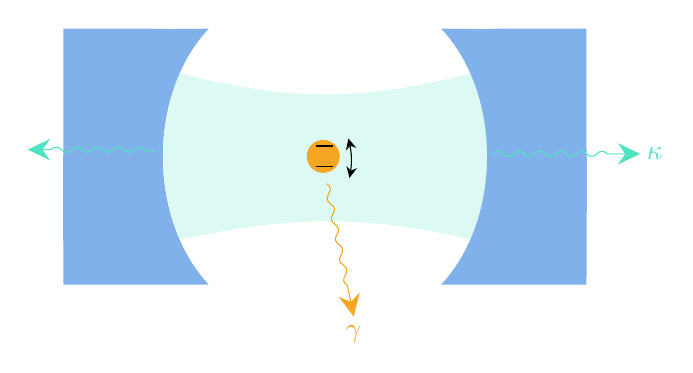
\begin{tikzpicture}[x=0.75pt,y=0.75pt,yscale=-1,xscale=1]
%uncomment if require: \path (0,300); %set diagram left start at 0, and has height of 300

%Shape: Polygon Curved [id:ds9510861200772092] 
\draw  [draw opacity=0][fill={rgb, 255:red, 74; green, 144; blue, 226 }  ,fill opacity=0.7 ] (80,28.7) .. controls (150.83,28.48) and (107.5,29.14) .. (150,28.7) .. controls (120.5,60.03) and (120.5,120.36) .. (150,152) .. controls (108.83,152.03) and (140.83,152.03) .. (80,152) .. controls (79.5,30.14) and (80.17,151.14) .. (80,28.7) -- cycle ;
%Shape: Polygon Curved [id:ds7955627052687326] 
\draw  [draw opacity=0][fill={rgb, 255:red, 74; green, 144; blue, 226 }  ,fill opacity=0.7 ] (332,28.7) .. controls (261.17,28.48) and (304.5,29.14) .. (262,28.7) .. controls (291.5,60.03) and (291.5,120.36) .. (262,152) .. controls (303.17,152.03) and (271.17,152.03) .. (332,152) .. controls (332.5,30.14) and (331.83,151.14) .. (332,28.7) -- cycle ;
%Shape: Polygon Curved [id:ds5301807467216497] 
\draw  [draw opacity=0][fill={rgb, 255:red, 80; green, 227; blue, 194 }  ,fill opacity=0.2 ] (135.87,50.17) .. controls (189.67,63.77) and (224.07,63.77) .. (276.07,50.17) .. controls (288.47,78.57) and (286.47,104.97) .. (276.07,130.17) .. controls (223.27,118.17) and (190.07,118.97) .. (136.27,130.17) .. controls (125.67,106.17) and (125.67,76.57) .. (135.87,50.17) -- cycle ;
%Shape: Circle [id:dp8724748988027644] 
\draw  [color={rgb, 255:red, 245; green, 166; blue, 35 }  ,draw opacity=1 ][fill={rgb, 255:red, 245; green, 166; blue, 35 }  ,fill opacity=1 ] (197.53,90.23) .. controls (197.53,86) and (200.97,82.57) .. (205.2,82.57) .. controls (209.43,82.57) and (212.87,86) .. (212.87,90.23) .. controls (212.87,94.47) and (209.43,97.9) .. (205.2,97.9) .. controls (200.97,97.9) and (197.53,94.47) .. (197.53,90.23) -- cycle ;
%Straight Lines [id:da7869724900400308] 
\draw    (201.53,85.23) -- (209.67,85.23) ;
%Straight Lines [id:da09643523980366409] 
\draw    (201.53,95.23) -- (209.67,95.23) ;
%Curve Lines [id:da42973004769989376] 
\draw    (218.33,97.59) .. controls (219.04,92.85) and (218.89,88.95) .. (217.96,84.46) ;
\draw [shift={(217.29,81.61)}, rotate = 75.47] [fill={rgb, 255:red, 0; green, 0; blue, 0 }  ][line width=0.08]  [draw opacity=0] (5.36,-2.57) -- (0,0) -- (5.36,2.57) -- (3.56,0) -- cycle    ;
\draw [shift={(217.79,100.61)}, rotate = 281.69] [fill={rgb, 255:red, 0; green, 0; blue, 0 }  ][line width=0.08]  [draw opacity=0] (5.36,-2.57) -- (0,0) -- (5.36,2.57) -- (3.56,0) -- cycle    ;
%Straight Lines [id:da3979605963713817] 
\draw [color={rgb, 255:red, 80; green, 227; blue, 194 }  ,draw opacity=1 ]   (287,89) .. controls (288.67,87.33) and (290.33,87.33) .. (292,89) .. controls (293.67,90.67) and (295.33,90.67) .. (297,89) .. controls (298.67,87.33) and (300.33,87.33) .. (302,89) .. controls (303.67,90.67) and (305.33,90.67) .. (307,89) .. controls (308.67,87.33) and (310.33,87.33) .. (312,89) .. controls (313.67,90.67) and (315.33,90.67) .. (317,89) .. controls (318.67,87.33) and (320.33,87.33) .. (322,89) .. controls (323.67,90.67) and (325.33,90.67) .. (327,89) .. controls (328.67,87.33) and (330.33,87.33) .. (332,89) .. controls (333.67,90.67) and (335.33,90.67) .. (337,89) .. controls (338.67,87.33) and (340.33,87.33) .. (342,89) -- (346.83,89) -- (354.83,89) ;
\draw [shift={(357.83,89)}, rotate = 180] [fill={rgb, 255:red, 80; green, 227; blue, 194 }  ,fill opacity=1 ][line width=0.08]  [draw opacity=0] (10.72,-5.15) -- (0,0) -- (10.72,5.15) -- (7.12,0) -- cycle    ;
%Straight Lines [id:da12077485396620125] 
\draw [color={rgb, 255:red, 80; green, 227; blue, 194 }  ,draw opacity=1 ]   (124,87) .. controls (122.33,88.67) and (120.67,88.67) .. (119,87) .. controls (117.33,85.33) and (115.67,85.33) .. (114,87) .. controls (112.33,88.67) and (110.67,88.67) .. (109,87) .. controls (107.33,85.33) and (105.67,85.33) .. (104,87) .. controls (102.33,88.67) and (100.67,88.67) .. (99,87) .. controls (97.33,85.33) and (95.67,85.33) .. (94,87) .. controls (92.33,88.67) and (90.67,88.67) .. (89,87) .. controls (87.33,85.33) and (85.67,85.33) .. (84,87) .. controls (82.33,88.67) and (80.67,88.67) .. (79,87) .. controls (77.33,85.33) and (75.67,85.33) .. (74,87) -- (73.83,87) -- (65.83,87) ;
\draw [shift={(62.83,87)}, rotate = 360] [fill={rgb, 255:red, 80; green, 227; blue, 194 }  ,fill opacity=1 ][line width=0.08]  [draw opacity=0] (10.72,-5.15) -- (0,0) -- (10.72,5.15) -- (7.12,0) -- cycle    ;
%Straight Lines [id:da46210121402694737] 
\draw [color={rgb, 255:red, 245; green, 166; blue, 35 }  ,draw opacity=1 ]   (206.83,103.36) .. controls (208.8,104.66) and (209.13,106.29) .. (207.83,108.26) .. controls (206.52,110.23) and (206.85,111.86) .. (208.82,113.16) .. controls (210.79,114.46) and (211.12,116.09) .. (209.82,118.06) .. controls (208.51,120.03) and (208.84,121.66) .. (210.81,122.96) .. controls (212.78,124.26) and (213.11,125.89) .. (211.81,127.86) .. controls (210.51,129.83) and (210.84,131.46) .. (212.81,132.76) .. controls (214.78,134.06) and (215.11,135.69) .. (213.8,137.66) .. controls (212.5,139.63) and (212.83,141.26) .. (214.8,142.56) .. controls (216.77,143.86) and (217.1,145.49) .. (215.79,147.46) .. controls (214.49,149.43) and (214.82,151.06) .. (216.79,152.36) -- (217.64,156.58) -- (219.24,164.42) ;
\draw [shift={(219.83,167.36)}, rotate = 258.52] [fill={rgb, 255:red, 245; green, 166; blue, 35 }  ,fill opacity=1 ][line width=0.08]  [draw opacity=0] (10.72,-5.15) -- (0,0) -- (10.72,5.15) -- (7.12,0) -- cycle    ;

% Text Node
\draw (359.83,89) node [anchor=west] [inner sep=0.75pt]  [color={rgb, 255:red, 80; green, 227; blue, 194 }  ,opacity=1 ] [align=left] {$\displaystyle \kappa $};
% Text Node
\draw (219.83,170.36) node [anchor=north] [inner sep=0.75pt]  [color={rgb, 255:red, 245; green, 166; blue, 35 }  ,opacity=1 ] [align=left] {$\displaystyle \gamma $};


\end{tikzpicture}

\end{center}

\textbf{Coupling with the environment} \begin{itemize}
    \item Cavity leaking $\kappa$
    \item Atomic spontaneous emission rate (outside the cavity) $\gamma$
    \item (Possible non-radiative decay: phonon, etc.)
\end{itemize}

\textbf{Strong coupling limit} $\kappa, \gamma \ll {\vb*{d} \cdot \vb*{E}_{\text{cavity}}}$ $\Rightarrow$ cavity QED

\end{frame}

\begin{frame}
\frametitle{Jaynes-Cummings model}

\begin{columns}
    \begin{column}{0.5\textwidth}
        \begin{itemize}
        \item No atom-atom interaction
        \item Rotating-wave approx.
        \item Single active photon mode
        \item No damping at all
        \end{itemize}
    \end{column}
    \begin{column}{0.5\textwidth}
        \begin{center}
            \tikzset{every picture/.style={line width=0.75pt}} %set default line width to 0.75pt        

            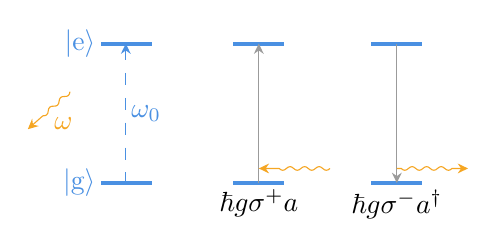
\begin{tikzpicture}[x=0.75pt,y=0.75pt,yscale=-0.7,xscale=0.7]
            %uncomment if require: \path (0,300); %set diagram left start at 0, and has height of 300
            
            %Straight Lines [id:da7090674543765305] 
            \draw [color={rgb, 255:red, 74; green, 144; blue, 226 }  ,draw opacity=1 ][line width=1.5]    (81.23,63.61) -- (116.29,63.61) ;
            %Straight Lines [id:da7959123856005688] 
            \draw [color={rgb, 255:red, 74; green, 144; blue, 226 }  ,draw opacity=1 ][line width=1.5]    (81.23,159.55) -- (116.29,159.55) ;
            %Straight Lines [id:da2804675610632261] 
            \draw [color={rgb, 255:red, 74; green, 144; blue, 226 }  ,draw opacity=1 ] [dash pattern={on 4.5pt off 4.5pt}]  (98.29,66.61) -- (98.29,159.55) ;
            \draw [shift={(98.29,63.61)}, rotate = 90] [fill={rgb, 255:red, 74; green, 144; blue, 226 }  ,fill opacity=1 ][line width=0.08]  [draw opacity=0] (7.14,-3.43) -- (0,0) -- (7.14,3.43) -- (4.74,0) -- cycle    ;
            %Straight Lines [id:da058635042932828174] 
            \draw [color={rgb, 255:red, 74; green, 144; blue, 226 }  ,draw opacity=1 ][line width=1.5]    (172.29,63.61) -- (207.36,63.61) ;
            %Straight Lines [id:da36096393830865026] 
            \draw [color={rgb, 255:red, 74; green, 144; blue, 226 }  ,draw opacity=1 ][line width=1.5]    (172.29,159.55) -- (207.36,159.55) ;
            %Straight Lines [id:da5936355014946022] 
            \draw [color={rgb, 255:red, 155; green, 155; blue, 155 }  ,draw opacity=1 ]   (189.83,159.55) -- (189.83,66.61) ;
            \draw [shift={(189.83,63.61)}, rotate = 90] [fill={rgb, 255:red, 155; green, 155; blue, 155 }  ,fill opacity=1 ][line width=0.08]  [draw opacity=0] (7.14,-3.43) -- (0,0) -- (7.14,3.43) -- (4.74,0) -- cycle    ;
            %Straight Lines [id:da6295417763364728] 
            \draw [color={rgb, 255:red, 245; green, 166; blue, 35 }  ,draw opacity=1 ]   (238.83,149.55) .. controls (237.16,151.22) and (235.5,151.22) .. (233.83,149.55) .. controls (232.16,147.88) and (230.5,147.88) .. (228.83,149.55) .. controls (227.16,151.22) and (225.5,151.22) .. (223.83,149.55) .. controls (222.16,147.88) and (220.5,147.88) .. (218.83,149.55) .. controls (217.16,151.22) and (215.5,151.22) .. (213.83,149.55) .. controls (212.16,147.88) and (210.5,147.88) .. (208.83,149.55) .. controls (207.16,151.22) and (205.5,151.22) .. (203.83,149.55) -- (200.83,149.55) -- (192.83,149.55) ;
            \draw [shift={(189.83,149.55)}, rotate = 360] [fill={rgb, 255:red, 245; green, 166; blue, 35 }  ,fill opacity=1 ][line width=0.08]  [draw opacity=0] (7.14,-3.43) -- (0,0) -- (7.14,3.43) -- (4.74,0) -- cycle    ;
            %Straight Lines [id:da5062719606323727] 
            \draw [color={rgb, 255:red, 74; green, 144; blue, 226 }  ,draw opacity=1 ][line width=1.5]    (267.29,63.61) -- (302.36,63.61) ;
            %Straight Lines [id:da8760493232717965] 
            \draw [color={rgb, 255:red, 74; green, 144; blue, 226 }  ,draw opacity=1 ][line width=1.5]    (267.29,159.55) -- (302.36,159.55) ;
            %Straight Lines [id:da5721160115969006] 
            \draw [color={rgb, 255:red, 155; green, 155; blue, 155 }  ,draw opacity=1 ]   (284.83,156.55) -- (284.83,63.61) ;
            \draw [shift={(284.83,159.55)}, rotate = 270] [fill={rgb, 255:red, 155; green, 155; blue, 155 }  ,fill opacity=1 ][line width=0.08]  [draw opacity=0] (7.14,-3.43) -- (0,0) -- (7.14,3.43) -- (4.74,0) -- cycle    ;
            %Straight Lines [id:da34204556310305745] 
            \draw [color={rgb, 255:red, 245; green, 166; blue, 35 }  ,draw opacity=1 ]   (330.83,149.55) -- (322.83,149.55) .. controls (321.16,151.22) and (319.5,151.22) .. (317.83,149.55) .. controls (316.16,147.88) and (314.5,147.88) .. (312.83,149.55) .. controls (311.16,151.22) and (309.5,151.22) .. (307.83,149.55) .. controls (306.16,147.88) and (304.5,147.88) .. (302.83,149.55) .. controls (301.16,151.22) and (299.5,151.22) .. (297.83,149.55) .. controls (296.16,147.88) and (294.5,147.88) .. (292.83,149.55) .. controls (291.16,151.22) and (289.5,151.22) .. (287.83,149.55) -- (284.83,149.55) -- (284.83,149.55) ;
            \draw [shift={(333.83,149.55)}, rotate = 180] [fill={rgb, 255:red, 245; green, 166; blue, 35 }  ,fill opacity=1 ][line width=0.08]  [draw opacity=0] (7.14,-3.43) -- (0,0) -- (7.14,3.43) -- (4.74,0) -- cycle    ;
            %Straight Lines [id:da1605315683236861] 
            \draw [color={rgb, 255:red, 245; green, 166; blue, 35 }  ,draw opacity=1 ]   (59.83,96.7) .. controls (59.7,99.05) and (58.45,100.16) .. (56.1,100.02) .. controls (53.75,99.89) and (52.5,101) .. (52.37,103.35) .. controls (52.24,105.7) and (50.99,106.81) .. (48.64,106.68) .. controls (46.29,106.54) and (45.04,107.65) .. (44.9,110) .. controls (44.77,112.35) and (43.52,113.46) .. (41.17,113.33) -- (39.04,115.23) -- (33.06,120.55) ;
            \draw [shift={(30.83,122.55)}, rotate = 318.29] [fill={rgb, 255:red, 245; green, 166; blue, 35 }  ,fill opacity=1 ][line width=0.08]  [draw opacity=0] (7.14,-3.43) -- (0,0) -- (7.14,3.43) -- (4.74,0) -- cycle    ;
            
            % Text Node
            \draw (79.23,159.55) node [anchor=east] [inner sep=0.75pt]  [color={rgb, 255:red, 74; green, 144; blue, 226 }  ,opacity=1 ]  {$\ket{\text{g}}$};
            % Text Node
            \draw (79.23,63.61) node [anchor=east] [inner sep=0.75pt]  [color={rgb, 255:red, 74; green, 144; blue, 226 }  ,opacity=1 ]  {$\ket{\text{e}}$};
            % Text Node
            \draw (100.29,111.58) node [anchor=west] [inner sep=0.75pt]  [color={rgb, 255:red, 74; green, 144; blue, 226 }  ,opacity=1 ]  {$\omega _{0}$};
            % Text Node
            \draw (47.33,112.62) node [anchor=north west][inner sep=0.75pt]  [color={rgb, 255:red, 245; green, 166; blue, 35 }  ,opacity=1 ]  {$\omega $};
            % Text Node
            \draw (189.83,162.55) node [anchor=north] [inner sep=0.75pt]    {$\hbar g\sigma ^{+} a$};
            % Text Node
            \draw (284.83,162.55) node [anchor=north] [inner sep=0.75pt]    {$\hbar g\sigma ^{-} a^{\dagger }$};
            
            
            \end{tikzpicture}
            
        \end{center}
    \end{column}
\end{columns}

\[
    H^{\text{Jaynes-Cummings}} = \hbar \omega \left( a^\dag a + \frac{1}{2} \right) + 
    \frac{\hbar \omega_0 }{2} \sigma^z + 
    \hbar g (a \sigma^+ + a^\dag \sigma^-)
\]

\textbf{Possible external field driving} $\omega_0 \to \Delta = \omega_0 - \omega_{\text{drive}}$

\end{frame}

\begin{frame}[t]
\frametitle{Quantum Rabi oscillation}

\textbf{Quantum nature of the model} \begin{itemize}
    \item $\ket*{\text{e}} \stackrel{\text{Spontaneous emission}}{\to}   \ket*{\text{g}}$ (but not irreversible)
\end{itemize}

\textbf{Dressed state} $H^{\text{Jaynes-Cummings}}$ in $\{ \ket*{\text{g}, n+1}, \ket*{\text{e}, n} \}$ = 
\[
    \hbar \omega \left( n + \frac{1}{2} \right) - \frac{\hbar \omega_0}{2} + 
    \pmqty{
        \hbar \omega  & \hbar g \sqrt{n+1} \\
        \hbar g \sqrt{n+1} & \hbar \omega_0
    }
\]

\begin{columns}[T]
    \begin{column}{0.5\textwidth}
        \begin{itemize}
            \item Oscillation starting with $\ket*{\text{e}}$
            \item Markovian approx. fails
            \item We have experimental evidence \faHandPointRight
        \end{itemize}
    \end{column}
    \begin{column}{0.5\textwidth}
        \includegraphics[width=\textwidth]{figs/quantum-rabi-annotated.png}
    \end{column}
\end{columns}

\blfootnote{Fig. from S Haroche et al., RMP 73 565 (2001)}

\end{frame}


\begin{frame}
\frametitle{Collapse and revival}

\textbf{Start with $\ket*{\text{e}, \alpha}$?} $\ket*{\psi(t=0)} = \ket*{\text{e}} \otimes \ee^{- \frac{\abs*{\alpha}^2}{2}} 
\sum_{n=0}^{\infty} \frac{\alpha^n}{\sqrt{n!}} \underbrace{\ket*{\text{e}, n}}_{\leftrightarrow \ket*{\text{g}, n+1}}$

\begin{columns}[T]
    \begin{column}{0.7\textwidth}
        \[
            \begin{aligned}
                P_\text{e}(t) &= \frac{1}{2}\left[1+\mathrm{e}^{-|\alpha|^2} \sum_{n=0}^{\infty} \frac{|\alpha|^{2 n}}{n !} \cos \left(\Omega_n t\right)\right] \\ 
                &\stackrel{t \ll 1 / g \abs*{\alpha}}{=} \frac{1}{2} + \frac{1}{2} \cos (2 g \abs{\alpha} t) \ee^{- \frac{1}{2} g^2 t^2}.
            \end{aligned}
        \]
        \textbf{Collapse of $P_{\text{e}}$ when $t \ll 1 / g \abs*{\alpha}$} 
        Because $\phi^{\ket*{\text{e},n}}$ not synchronized
        
        This can be simulated by a thermalized state as well; but as $\ket*{\psi}$ is not truly incoherent\dots 
    \end{column}
    \begin{column}{0.3\textwidth}
        \vspace{0.2cm}
        \includegraphics[width=\textwidth]{figs/coherent-different-phases.png}
    \end{column}
\end{columns}

\end{frame}

\begin{frame}
\frametitle{Collapse and revival}

\textbf{Revival} When the phases of the major components realign again: $2\pi = (\Omega_{\abs*{\alpha}} - \Omega_{\abs*{\alpha}^2 - 1}) t$

\begin{columns}[T]
    \begin{column}{0.6\textwidth}
        \begin{center}
            \includegraphics[width=\textwidth]{figs/collapse-revival.PNG}
    \end{center}
    \end{column}
    \begin{column}{0.4\textwidth}
        Revival is a
        \begin{itemize}
            \item Coherent property: not possible in a thermalized state
            \item ``granular'' property: see $\abs*{\alpha}^2-1$ 
        \end{itemize} 
    \end{column}
\end{columns}

\blfootnote{Fig. from arXiv 1111.1143.}

\end{frame}

\begin{frame}
\frametitle{Creation of entangled atom pairs}

\textbf{Protocol}
\begin{enumerate}
    \item Move atom 1 (in $\ket*{\text{e}}$) into the cavity mode. 
    \item $\ket*{\text{e}_1, 0} \stackrel{\frac{1}{2} \Omega_0 t = \frac{\pi}{4}}{\longrightarrow} \frac{1}{\sqrt{2}} (\ket*{\text{g}_1, 1} + \ket*{\text{e}_1, 0})$.
    \item Move atom 1 out of the light beam. Move atom 2 (in $\ket*{\text{g}}$) into the light beam.
    \item $\frac{1}{\sqrt{2}} (\ket*{\text{g}_1, \underbrace{\text{g}_2, 1}_{\mathclap{\text{coupling happens only here}}}} + \ket*{\text{e}_1, \text{g}_2, 0}) 
    \stackrel{\frac{1}{2} \Omega_0 t = \frac{\pi}{2}}{\longrightarrow} 
    \frac{1}{\sqrt{2}} (\ket*{\text{g}_1, \text{e}_2, 0} + \ket*{\text{e}_1, \text{g}_2, 0})$
    \item Move all atoms out. 
\end{enumerate}

That's how you get an Einstein-Podolsky-Rosen pair.

\end{frame}

\title{Cavity and medium}
\author{}
\date{}

\begin{frame}[noframenumbering,plain]
    \titlepage
\end{frame}

\begin{frame}
\frametitle{``Usual'' medium within cavity?}

The full theory of quantum optics with $\epsilon(\omega)$ is \emph{hard}!!!

\textbf{In a theory only about photons: $\epsilon(\omega)$ $\Rightarrow$ $\Im \epsilon \neq 0$ $\Rightarrow$ non-unitary?}

\begin{enumerate}
    \item Auxiliary fields needed for frequency dependence
    \item $\Rightarrow$ (space-resolved) Input-output formalism
    \item $\stackrel{\text{thermalization}}{\Rightarrow}$ quantum Langevin eq.
\end{enumerate}

\vspace{0.4cm}

\textbf{Alternatively we pick up excitations in the medium as auxiliary fields, or ``atoms''}

\blfootnote{See e.g. arXiv quant-ph/0006121, PRL 110, 153602}

\end{frame}

\begin{frame}
\frametitle{Cavity QED with exciton}

\begin{columns}[T]
    \begin{column}{0.45\textwidth}
        \textbf{Setup}
        \begin{itemize}
            \item One active photon mode
            \item Probing by the side
            \item Exciton modes (``two-level atom'': \xmark two excitons in one mode)
        \end{itemize}
    \end{column}
    \begin{column}{0.55\textwidth}
        \begin{center}
            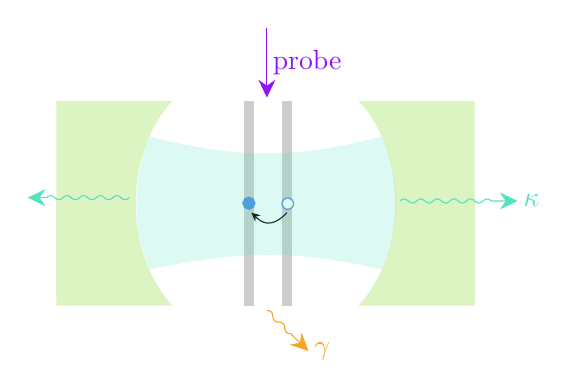
\begin{tikzpicture}[x=0.75pt,y=0.75pt,yscale=-0.8,xscale=0.8]
                %uncomment if require: \path (0,300); %set diagram left start at 0, and has height of 300
                
                %Shape: Polygon Curved [id:ds7921799041188771] 
                \draw  [draw opacity=0][fill={rgb, 255:red, 184; green, 233; blue, 134 }  ,fill opacity=0.5 ] (100,76.7) .. controls (170.83,76.48) and (127.5,77.14) .. (170,76.7) .. controls (140.5,108.03) and (140.5,168.36) .. (170,200) .. controls (128.83,200.03) and (160.83,200.03) .. (100,200) .. controls (99.5,78.14) and (100.17,199.14) .. (100,76.7) -- cycle ;
                %Shape: Polygon Curved [id:ds5672480064156658] 
                \draw  [draw opacity=0][fill={rgb, 255:red, 184; green, 233; blue, 134 }  ,fill opacity=0.5 ] (352,76.7) .. controls (281.17,76.48) and (324.5,77.14) .. (282,76.7) .. controls (311.5,108.03) and (311.5,168.36) .. (282,200) .. controls (323.17,200.03) and (291.17,200.03) .. (352,200) .. controls (352.5,78.14) and (351.83,199.14) .. (352,76.7) -- cycle ;
                %Straight Lines [id:da35194224521755535] 
                \draw [color={rgb, 255:red, 80; green, 227; blue, 194 }  ,draw opacity=1 ]   (307,137) .. controls (308.67,135.33) and (310.33,135.33) .. (312,137) .. controls (313.67,138.67) and (315.33,138.67) .. (317,137) .. controls (318.67,135.33) and (320.33,135.33) .. (322,137) .. controls (323.67,138.67) and (325.33,138.67) .. (327,137) .. controls (328.67,135.33) and (330.33,135.33) .. (332,137) .. controls (333.67,138.67) and (335.33,138.67) .. (337,137) .. controls (338.67,135.33) and (340.33,135.33) .. (342,137) .. controls (343.67,138.67) and (345.33,138.67) .. (347,137) .. controls (348.67,135.33) and (350.33,135.33) .. (352,137) .. controls (353.67,138.67) and (355.33,138.67) .. (357,137) .. controls (358.67,135.33) and (360.33,135.33) .. (362,137) -- (366.83,137) -- (374.83,137) ;
                \draw [shift={(377.83,137)}, rotate = 180] [fill={rgb, 255:red, 80; green, 227; blue, 194 }  ,fill opacity=1 ][line width=0.08]  [draw opacity=0] (10.72,-5.15) -- (0,0) -- (10.72,5.15) -- (7.12,0) -- cycle    ;
                %Straight Lines [id:da2876961165546532] 
                \draw [color={rgb, 255:red, 80; green, 227; blue, 194 }  ,draw opacity=1 ]   (144,135) .. controls (142.33,136.67) and (140.67,136.67) .. (139,135) .. controls (137.33,133.33) and (135.67,133.33) .. (134,135) .. controls (132.33,136.67) and (130.67,136.67) .. (129,135) .. controls (127.33,133.33) and (125.67,133.33) .. (124,135) .. controls (122.33,136.67) and (120.67,136.67) .. (119,135) .. controls (117.33,133.33) and (115.67,133.33) .. (114,135) .. controls (112.33,136.67) and (110.67,136.67) .. (109,135) .. controls (107.33,133.33) and (105.67,133.33) .. (104,135) .. controls (102.33,136.67) and (100.67,136.67) .. (99,135) .. controls (97.33,133.33) and (95.67,133.33) .. (94,135) -- (93.83,135) -- (85.83,135) ;
                \draw [shift={(82.83,135)}, rotate = 360] [fill={rgb, 255:red, 80; green, 227; blue, 194 }  ,fill opacity=1 ][line width=0.08]  [draw opacity=0] (10.72,-5.15) -- (0,0) -- (10.72,5.15) -- (7.12,0) -- cycle    ;
                %Straight Lines [id:da3223318165306617] 
                \draw [color={rgb, 255:red, 245; green, 166; blue, 35 }  ,draw opacity=1 ]   (226.83,202.96) .. controls (229.19,202.93) and (230.38,204.1) .. (230.41,206.46) .. controls (230.44,208.82) and (231.63,209.98) .. (233.99,209.95) .. controls (236.35,209.92) and (237.54,211.08) .. (237.57,213.44) .. controls (237.6,215.8) and (238.79,216.96) .. (241.15,216.93) -- (243.96,219.67) -- (249.69,225.26) ;
                \draw [shift={(251.83,227.35)}, rotate = 224.29] [fill={rgb, 255:red, 245; green, 166; blue, 35 }  ,fill opacity=1 ][line width=0.08]  [draw opacity=0] (10.72,-5.15) -- (0,0) -- (10.72,5.15) -- (7.12,0) -- cycle    ;
                %Straight Lines [id:da9541990650969336] 
                \draw [color={rgb, 255:red, 155; green, 155; blue, 155 }  ,draw opacity=0.5 ][line width=3.75]    (216,76.7) -- (216,200) ;
                %Straight Lines [id:da26115880911209577] 
                \draw [color={rgb, 255:red, 155; green, 155; blue, 155 }  ,draw opacity=0.5 ][line width=3.75]    (239,76.7) -- (239,200) ;
                %Straight Lines [id:da3174413100165303] 
                \draw [color={rgb, 255:red, 74; green, 144; blue, 226 }  ,draw opacity=1 ]   (216,138.35) ;
                \draw [shift={(216,138.35)}, rotate = 0] [color={rgb, 255:red, 74; green, 144; blue, 226 }  ,draw opacity=1 ][fill={rgb, 255:red, 74; green, 144; blue, 226 }  ,fill opacity=1 ][line width=0.75]      (0, 0) circle [x radius= 3.35, y radius= 3.35]   ;
                %Curve Lines [id:da05051086792467019] 
                \draw    (219.65,146.14) .. controls (223.52,149.9) and (229,154.2) .. (238.96,144.03) ;
                \draw [shift={(217.46,144.03)}, rotate = 41.19] [fill={rgb, 255:red, 0; green, 0; blue, 0 }  ][line width=0.08]  [draw opacity=0] (5.36,-2.57) -- (0,0) -- (5.36,2.57) -- (3.56,0) -- cycle    ;
                %Shape: Circle [id:dp4169653576240837] 
                \draw  [color={rgb, 255:red, 74; green, 144; blue, 226 }  ,draw opacity=1 ] (235.88,138.61) .. controls (235.88,136.68) and (237.44,135.11) .. (239.37,135.11) .. controls (241.31,135.11) and (242.87,136.68) .. (242.87,138.61) .. controls (242.87,140.55) and (241.31,142.11) .. (239.37,142.11) .. controls (237.44,142.11) and (235.88,140.55) .. (235.88,138.61) -- cycle ;
                %Shape: Circle [id:dp3040674509595094] 
                \draw  [color={rgb, 255:red, 255; green, 255; blue, 255 }  ,draw opacity=1 ][fill={rgb, 255:red, 255; green, 255; blue, 255 }  ,fill opacity=1 ] (236.88,138.61) .. controls (236.88,137.23) and (237.99,136.11) .. (239.37,136.11) .. controls (240.76,136.11) and (241.87,137.23) .. (241.87,138.61) .. controls (241.87,140) and (240.76,141.11) .. (239.37,141.11) .. controls (237.99,141.11) and (236.88,140) .. (236.88,138.61) -- cycle ;
                
                %Shape: Polygon Curved [id:ds3207245514060506] 
                \draw  [draw opacity=0][fill={rgb, 255:red, 80; green, 227; blue, 194 }  ,fill opacity=0.2 ] (155.87,98.17) .. controls (209.67,111.77) and (244.07,111.77) .. (296.07,98.17) .. controls (308.47,126.57) and (306.47,152.97) .. (296.07,178.17) .. controls (243.27,166.17) and (210.07,166.97) .. (156.27,178.17) .. controls (145.67,154.17) and (145.67,124.57) .. (155.87,98.17) -- cycle ;
                %Straight Lines [id:da13938461311970474] 
                \draw [color={rgb, 255:red, 144; green, 19; blue, 254 }  ,draw opacity=1 ]   (226.83,32.96) -- (226.83,71.7) ;
                \draw [shift={(226.83,74.7)}, rotate = 270] [fill={rgb, 255:red, 144; green, 19; blue, 254 }  ,fill opacity=1 ][line width=0.08]  [draw opacity=0] (10.72,-5.15) -- (0,0) -- (10.72,5.15) -- (7.12,0) -- cycle    ;
                
                % Text Node
                \draw (379.83,137) node [anchor=west] [inner sep=0.75pt]  [color={rgb, 255:red, 80; green, 227; blue, 194 }  ,opacity=1 ] [align=left] {$\displaystyle \kappa $};
                % Text Node
                \draw (253.83,227.35) node [anchor=west] [inner sep=0.75pt]  [color={rgb, 255:red, 245; green, 166; blue, 35 }  ,opacity=1 ] [align=left] {$\displaystyle \gamma $};
                % Text Node
                \draw (228.83,53.83) node [anchor=west] [inner sep=0.75pt]  [color={rgb, 255:red, 144; green, 19; blue, 254 }  ,opacity=1 ] [align=left] {probe};
                
                
                \end{tikzpicture}                
        \end{center}
    \end{column}
\end{columns} 

The effective theory: one photon mode, several atoms

\textbf{Why this matters} $\mel*{S}{\vb*{d}}{0} = 0 \nRightarrow \mel*{S_1}{\vb*{d}}{S_2} = 0$: dark excitons are optically active in this setting!

\end{frame}

\begin{frame}
\frametitle{Cavity QED with excitons as atoms}

\textbf{Exciton polariton} is $c_1 \ket*{\text{exciton}} + c_2 \ket*{\text{photon}}$ 

\begin{itemize}
    \item Easiest setup
    \item From the perspective of excitons: virtual photons only
\end{itemize}

\textbf{Optical spectrum} $\Omega$ = cavity mode freq., $\omega$ = detection freq. 

\begin{columns}[T]
    \begin{column}{0.5\textwidth}
        \includegraphics[width=\textwidth]{figs/cavity-exciton-polariton.PNG}
    \end{column}
    \begin{column}{0.5\textwidth}
        \begin{itemize}
            \item Dark modes appear (I)
            \item Quench of optical activity in one band (II) 
        \end{itemize}
    \end{column}
\end{columns}

\blfootnote{Fig. from Nano Letters 2019 19 (6), 3473-3479}

\end{frame}

\begin{frame}
\frametitle{Cavity QED with surface
plasmon polaritons (SPPs) as photons}

\begin{columns}[T]
    \begin{column}{0.7\textwidth}
        \textbf{Setup}
        \begin{itemize}
            \item Replace ``simple'' photons by SPPs.
            \item Atom = exciton on nanoparticle
        \end{itemize}
    \end{column}
    \begin{column}{0.3\textwidth}
        \includegraphics[width=\textwidth]{figs/emitter-in-sandwich.PNG}
    \end{column}
\end{columns}

\textbf{Rabi oscillation of excited state population} 
\begin{center}
    \includegraphics[width=0.6\textwidth]{figs/emitter-plasmon.PNG}
\end{center}

\blfootnote{PRB 89, 041402(R) (2014)}

\end{frame}

\begin{frame}
\frametitle{Take home message}

\begin{itemize}
    \item Cavity $\Rightarrow$ highly selective strong light-matter interaction $\Rightarrow$ high coherence $\Rightarrow$ necessity of cavity QED 
    \item Quantum Rabi oscillation, collapse and revival, entanglement
    \item Cavity QED happens everywhere
\end{itemize}

\end{frame}

\end{document}